%% note: todo's go in todo, as well as optionally in here

\section{Experiment Results}
For our initial experiments we test how well our system scales. We download a small file (100KB) 
under several different load settings. In each test a given number of peers enter the system within 
the first 100s, using a poisson distribution with an inter arrival time that is 100s/number of peers, 
so that they enter pseudo-randomly within the first 100s. Peers originally request the file from 
an origin server located on a well provisioned machine at BYU, using an Apache2 web server that it 
bandwidth limited (using mod\_bw) to 256KB/s. Peers are randomly selected from available PlanetLab 
hosts (a pool of up to 300 scattered world-wide on the PlanetLab system). Experiments run until 
all peers finish downloading the file. Each experiment is repeated 3 times and results are averaged. 
A different filename is used with each run, so as to not reuse the same DHT keys. We collect the download 
times of all peers in a run and calculate the 1st, 25th, 50th, 75th, and 99th percentiles. We also 
measure the amount of load on the origin server, measured as the sum of bytes received within a given 
second by peers, from the origin. This only measures bytes received from the origin, not bytes sent, 
as any data received after a socket has already been closed is ignored by TCP, and peer sometimes 
close connections early. We also calculate the amount of the file received from peers versus from 
the origin, as well as the time required to do the DHT get, put, and remove operations during each 
run.

We first test a traditional client-server transfer, to establish a base line from which to compare 
our system. Fig.~\ref{fig:client_server_download_times} shows the download times for client-server 
download, varying load. Median download times have a low of 1.33s with 1 peer entering the system/second, 
and quickly grows to a high of 344s at 20 peers/second. Download times increase linearly (instead 
of exponentially) because we start a fixed number of peers and let them all complete their downloads. 
The topmost outliers at 20s are peers which typically waited in line around 900s before finally 
being served the file. Load on the origin server grew quickly to its theoretical cap of 250KB/s (Fig.~\ref{fig:client_server_server_load}) 
at 3 peers/s. Under higher load (20 peers/s), server speed actually decreases to 203KB/s, which 
shows the limitations of our bandwidth limiter in that it becomes bursty at higher connection rates. 

\begin{figure*}
  \begin{center}
    \subfigure[Load on the origin server]{
      \includegraphics[width=7cm]{pics/vr_unnamed316651_cs_stress_test/server_speed_Percentile_Line.pdf}
      \label{fig:client_server_server_load}
    }
    \subfigure[Download times]{
      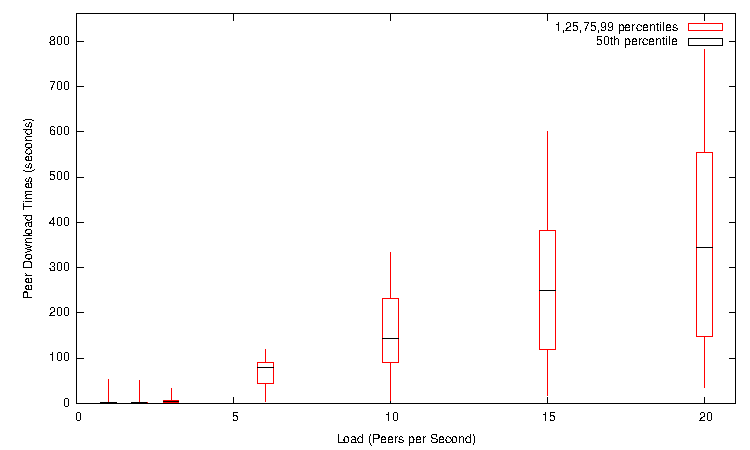
\includegraphics[width=7cm]{pics/vr_unnamed316651_cs_stress_test/client_download_Percentile_Line.pdf}
      \label{fig:client_server_download_times}      
    }     
    \caption{Traditional client server download}  
  \end{center}
\end{figure*}

We next test our system under the same loads. For system parameters, we chose reasonable defaults 
of a block size of 100KB, origin minimum allowed speed (R) of 128KB/s, R's calculation window (W) 
of 2s, and first-byte timeout (T) of 1s. Peers linger, serving the file, for 20 seconds after completing 
a download, and download from at most 5 others peers at a time. Results are that download median times 
(Fig. \ref{fig:yanc_download_times}) start at 1.4s at 1 peer entering the system/second, grow 
to 5.23s at 6 peers/s and 7.46s at 20 peers/s. The graph's Y axis for download time (Fig. \ref{fig:yanc_download_times}) 
is different than that for client-server (Fig.~\ref{fig:client_server_download_times}) 
because the difference is so great that it would obscure the lines. At a load of 20 peers/s 99.5\% 
of peers took one second (T) to give up on the origin server, because of not having received a response 
byte. They then query the DHT for a peer list, and receive a response with a median latency of 5.215s, 
and then download the file almost immediately, hence the median of about 7s. Of those that took longer 
there are two basic causes. One was that poorly connected peers would take so long to download a file 
that the linger times of peers serving it to them would expire. They would then have to request a new 
list of peers, causing an increase in latency. This problem was exacerbated by the fact that we request 
the last block from multiple peers, in order to download the last block more efficiently. This causes 
some redundancy in bytes received, which slows down slow peers, causing them to timeout their peer 
connections more often. The other factor causing slowdown is a sometimes unresponsive DHT. We 
set DHT requests to timeout after 60s if no response was received--a reasonable value to keep from 
overloading the DHT. Typically requests came back quickly, however at times they would timeout, 
andpeers would end up downloading the entire file from an (overloaded) origin, or perform a new 
query after 60s, and then quickly download the file after that. 
The amount received from the origin decreases with higher load, mostly because mod\_bw serves 
very little when it is under high load, but also because the peers receive the file much more quickly 
from their peers (Fig. \ref{fig:yanc_origin_server_load}). 
<%= figure_directory 'vr_medium_p2p_load_tak4', 'yanc', 'P2P results varying load' %>

The amount of P2P transfer also increases under higher loads. Under low load peers tend to download 
the file only from the origin, however, after about 10 peers/s almost 100\% of the transfer is being 
done from peers (Fig.~\ref{fig:yanc_cdf_from_peers}--a 1 on the graph means 100\% of the file 
transfer is from peers). The reason it isn't always at 100\% for lower load levels is that peers start 
downloading the file from the origin, receive some portion of it within the first W (2) seconds, 
then transition to P2P and receive the rest, hence it being a lower percentage of transfer under 
higher load levels. The fastest percentile almost always download the entire file from the origin 
(typically the first few peers to enter the system), and later peers almost always download the 
file using p2p, because they encounter a bogged down origin server. 
\section{Impact of various parameters}

Theoretically, if a peer can download from a fast origin, it does not need to download the file from 
peers. Our system allows for this by specifying parameters for the conditions under which it will 
``give up" on the origin and switch to p2p download\footnote{Note that it actually switches to 
a mixed download, since it still downloads from the origin server if no peers are available.}. We 
next test the impact of varying these transition parameters, as well as other settings, in order 
to explore the dynamics of the system. In each test we run 1000 peers, with an average of 15 peers entering 
the system per second, using a poisson distribution with an interarrival time of 0.066s. We then 
wait for all peers to finish downloading. The download a 100KB file, with a block size of 100KB, from 
at most 20 peers simultaneously. T is set by default to 1s, R to 128KB/s, and W to 2s. 
\subsection{Time to wait for first byte T}

We first test varying $T$, the timeout for a first response byte from the origin server\footnote{By 
first byte we mean any byte received from the origin server--a header byte or a content byte--i.e. 
we exclude the TCP handshake packet as counting as a first byte.}. We expect that an extremely low value will cause transitioning too early and an extremely high value 
will cause transitioning too late. The results held to our hypothesis for low values but not for 
high. With a T setting of 0s, median download time was 12s. It then dropped to 4.5s with T set at 0.75s, 
and rose to 10s with T set at 2s, and then flattens out for higher values (Fig. \ref{fig:vary_t_download_times}). 
The reason it flattens out with higher values was that T's relative importance decreases when it 
is high, and R causes the transition more often (Fig. \ref{fig:vary_t_death_reasons}). With 
low values of T, almost 100\% of peers transitioned to P2P download because of T. With T set at 10 seconds 
about 80\% of peers transitioned because of T, and 20\% because of R. 
%The outliers for download time are usually peers who were poorly connected to the DHT, so they sometimes 
received answers to their queries after the answers were already outdated, so had trouble connecting 
to live peers. 
<%= figure_directory 'vr_unnamed17712_dT', 'vary_t', 'Varying T', true %>

\subsection{Server minimum allowed speed R}

We next examine the effect of varying $R$, the server speed's minimum cut off. This value is calculated 
by summing the amount received from the origin over the previous W seconds (set to 2). W is calculated 
starting from the time a first byte is received. We vary R from 32KB/s to 1MB/s, and leave T set to a 
reasonably high value of 10s. The expected result was that a value of R too high would cause transition 
too early, and that a value too low would cause a transition too late. This was the case, as with R set 
to 5K, median download times are 40s, with R at 40K, download times dropped to 15s, and they reached 
a low of 13s with R set to 160K. Higher values than 160K resulted in slowdown, with R set to 1MB having 
a median download time of 30s (Fig.~\ref{fig:vary_dr_download_times}). 
<%= figure_directory 'vr_unnamed502788_dR_fromStart_5000by_fixed_settingAndMajorTimes_8_times_0.0666666666666667s__10s_100000B_255000BPS_5000s_10s_2.0s_100000B', 'vary_dr', 'Varying R' %> 

\subsection{Server speed time window W}

We next vary W, the amount of recent download history used to calculate R. Our hypothesis is that 
a small value for W will cause calculation to be too sensitive and cause slowdown. We vary W from 0.1s 
to 10s and run the experiment described above with T set to 10s and R set to 128KB/s. The results are 
slightly different than our hypothesis. Varying W does make some difference, but only when set 
to a very low value. Median download times are 17s with W set to 0.25s. For W \textgreater{} 0.25s 
median download times stayed at around 25s (Fig.~\ref{fig:dw_download_times}). Surprisingly, 
most peers (consistently about 800 out of 1000) still transitioned to a P2P download because of 
a slow first byte (T), even with T set to the larger value of 10s (Fig.~\ref{fig:dw_death_reasons}). 
The reason for this is that we don't start calculating R until after the first byte is received, and 
in the majority of cases (800/1000) this didn't happen until after T had expired, at 10s, so T still 
causes most of the P2P transitioning. A lower value of W made for faster downloads because the first 
200 peers, who do receive bytes from the origin, transition more quickly to P2P download. 
% ltodo so was it all the first 200 that always transitioned to R, so that's what sped things up a bit?

% why was this higher, then?

<%= figure_directory '837145_dw', 'dw', 'Varying W', true %>

\section{Effect for a full web page}

We next run an experiment more indicative of real-world situations. The normal pattern for a web 
page download is to first access some root page which references several others, such as images, 
javascript, flash, etc. This is the case for the BYU web site, which has a medium sized main page that 
links to over 10 small other objects\footnote{Snapshot 2007}. We therefore next run an experiment 
to see how well our system downloads a small page followed by several smaller files. Each peer first 
downloads a 100K file. When that file completes each peer then downloads 10 10K files simultaneously 
(all from the origin server), and the total time to download all 11 files is measured. We set the parameters 
to be those mentioned above, and run 1000 peers, varying the load on the origin from 1 peer/s to 25 
peers/s. 
The expected result is that downloading multiple pages will be slower than downloading only one 
since it will put more stress on the DHT, which proved correct (Fig. \ref{fig:multiple_files_download_times_all_files}). 
Total download time starts at 1.3s, and appears to grow dramatically with increased load, approaching 
150s total download time at 25 peers/s. Also correlated is that DHT times grow with load, starting 
at a median of 0.41s at 1 peer/s for put queries, and growing to a median of 12s/query at 25 peers/s 
(Fig. \ref{fig:multiple_files_p2p_dht_put}). Because we are downloading 11 files instead 
of 1, download time increases. Also interesting to note is the load on the origin server (Fig. \ref{fig:multiple_files_origin_server_load}). 
It goes down when there are about 10 peers per second (most of the download is being down via P2P), 
however, at higher loads, it increases as our system is not able to handle the strain of more peers. 

% todo is that what really happens though?

\begin{figure*}\begin{center} 
 \subfigure[Load on the origin server] {
  \includegraphics[width=70mm,]{pics/vr_multiples_take_1/server_speed_Percentile_Line.pdf}
  \label{fig:multiple_files_origin_server_load}
 } 
 \subfigure[Download times] {
  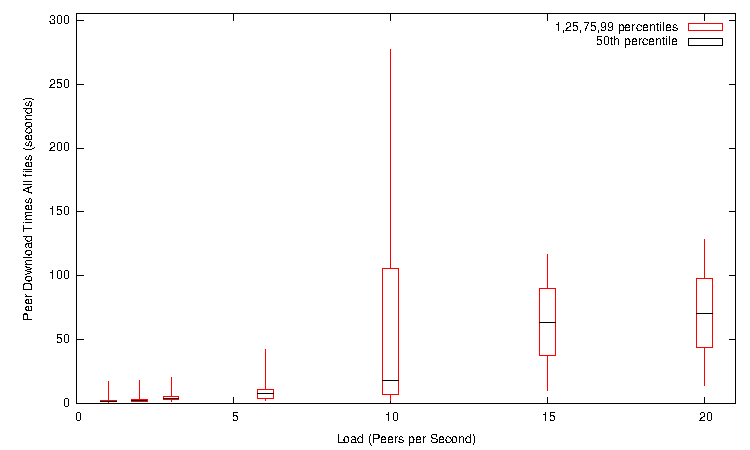
\includegraphics[width=70mm,]{pics/vr_multiples_take_1/client_download_all_files_Percentile_Line.pdf}
  \label{fig:multiple_files_download_times_all_files}
 } 
 \subfigure[CDF of percent of file received from peers] {
  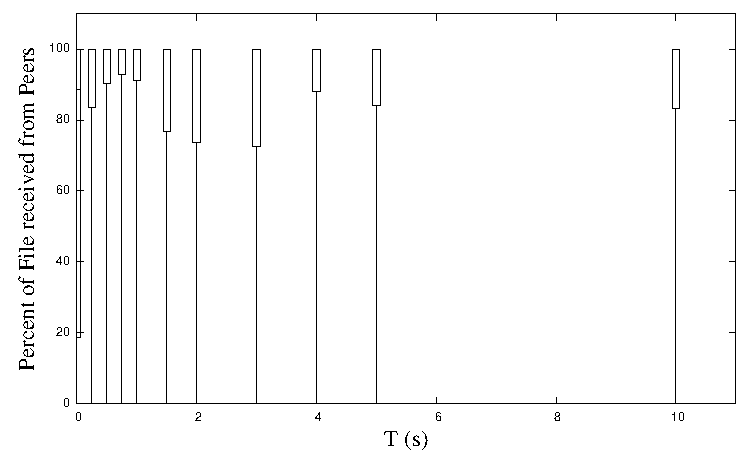
\includegraphics[width=70mm,]{pics/vr_multiples_take_1/percent_from_clients_Percentile_Line.pdf}
  \label{fig:multiple_files_cdf_from_peers}
 }
 \subfigure[DHT put times] {
  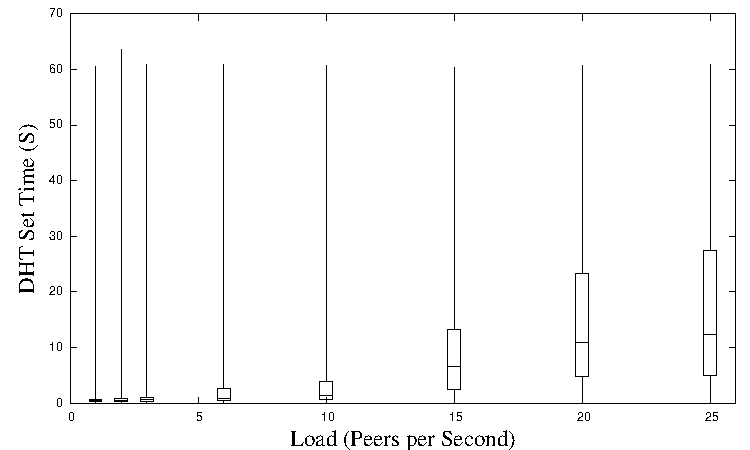
\includegraphics[width=70mm,]{pics/vr_multiples_take_1/dht_Put_Percentile_Line.pdf}  
  \label{fig:multiple_files_p2p_dht_put}
 }
    \caption[]{Downloading multiple simultaneous files}
    \end{center}
    \end{figure*}

We next re-run the same test using a traditional client-server download. Download times using 
client-server only grew at a much steeper rate (Fig. \ref{fig:multiple_files_cs_download_times}). 

<%= figure 'pics/multiples_p2p_versus_cs_pics/client_download_Percentile_Line.pdf', :caption => 'Comparison of P2P versus client server download times for multiple files', :label => 'fig:multiple_files_cs_download_times' %> 
\subsection{Varying Block Size}

We next measure the effect block size has on downloads. We download a 100K file with block sizes from 
16KB to 100KB. We run 1000 peers at an average of 15 peers entering per second. 32K blocks resulted 
in the quickest downloads (10.6s median) (Fig.~\ref{fig:vary_block_size_download_times}). 

%32KB blocks were shown to be effective in \cite{TODO}.  

<%= figure_directory 'vr_unnamed240998_blockSize', 'vary_block_size', 'Varying block size' %>

\section{Downloading Large Files}

We next test our system's ability to download large files. We download a 30MB file with 100 peers, 
using the same settings as the above, and then download the same file, using BitTorrent, with similar 
settings. Block size is set to 256K for both systems. Peers enter the system at an average of 1/s, 
and both protocols' origin servers are rate limited to 256KB/s. With both systems, linger time 
is set to 0s. The expected result is that the two fare similarly. It turned out that a few peers download 
faster with our system, but most download faster with BitTorrent (Table~\ref{fig:yanc_vs_bt}). 
Ours had a slower median than BitTorrent (847s to 148s), though BitTorrent was worse for the 99th 
percentile (2786s to 847s). We're not entirely sure exactly what makes BitTorrent faster.  One reason for the difference is that the BitTorrent's seed 
limits the number of outgoing connections it will entertain to 7 (Apache--our server--does 
too, but to 256). This limit enables BitTorrent to propagate blocks more quickly to peers, who then 
spread the blocks among the other peers. BitTorrent seeds also favor peers who have higher download 
speeds, which helps speed propagation of blocks. For our test BitTorrent uses a dedicated tracker, 
which also made peer rendezvous quicker than using our DHT.  It also uses a ``rarest block first" policy in block selection, enabling it to share blocks more efficiently.  These differences combined allow it 
to respond to a flash crowd such as this one better.  In future work we will optimize our system to handle flash crowds such as this one better, by backing off more on the origin server.  One interesting statistic is the relative download percentiles. The difference between 25th and 75th percentiles of our system is about 150s, 
or 5\% of the 75th percentile's time. The difference between the 25th and 75th percentiles of BitTorrent 
is 24s, or about 7\%. These numbers being close means that once a few of the peers have downloaded 
the file, it doesn't take (relatively) long in either system for the rest of the peers to complete 
the download (Fig.~\ref{fig:yanc_30mb_cdf}). Very few peers receive more than 50\% of the file 
from the origin (2\%). 
<%= figure 'pics/yanc_30mb/yanc_30_mb_cdf.pdf', :caption => 'CDF of percent of file received from peers, 30MB file', :label => 'fig:yanc_30mb_cdf' %>

\begin{table}
  \caption{Download times of a 30MB file}
\begin{tabular}{ c c l }
  Percentiles & Our System (S) & BitTorrent (S) \\
  \hline
  1 & 613 & 131 \\
  25 & 730 & 139 \\
  50 & 847 & 148 \\
  75 & 882 & 163 \\
  99 & 982 & 2786 \\
  \label{fig:yanc_vs_bt}
\end{tabular}
\end{table}
  
\section{Peer connection limit} 

We next vary the maximum number of download connections each peer is allowed to have at a time. We 
repeat the previous (30MB file size) experiment, but vary the peer connection limit from 1 to 50. 
We expect that download times will suffer if the connection limit is too low. As expected, median 
download times suffered with a low connection limit, with a peak time of 1604s with a limit of 1. Download 
times decreased with a higher connection limit, with 16 yielding a median download time of 931s 
(Fig. \ref{fig:vary_connection_count_download_times}), however limits greater than 16 didn't 
yield much relative gain. A 50 peer limit resulted in a median download time of 875s. 
<%= figure_directory 'vr_vary_blocks_large_file', 'vary_connection_count', 'Varying number of concurrent peers' %>

\section{Varying linger time}

We next vary the amount of (post file download) linger time, our hypothesis being that a longer linger 
time will increase download speeds, which proved correct (Fig.~\ref{fig:vary_linger_time_download_times}). 
We download a 100K file (using the same parameters as the original T test) varying linger time. The 
results confirm our hypothesis. With a linger time of 0s, median download time was near 300s, with 
a median download time of 127s with linger time at 1s, 60s with linger 2s, 34s with linger time of 4s, 
and staying mostly constant for linger times greater than 4s. 
<%= figure_directory 'vr_unnamed497104_linger_fromStart_0by_fixed_settingAndMajorTimes_8_times_0.0666666666666667s__0s_100000B_255000BPS_125000s_1.0s_2.0s_100000B', 'vary_linger_time', 'Varying linger time' %> 
